\section{Experiments}
As a first experiment we can experiment with what happens when we change the values of \textit{f}, i.e. our grid values, and when we change $\kappa$ in our toy example. In the notebook we define $f = X+Y$ where \textit{X} and \textit{Y} are linear sequences of numbers. This defines a flat grid with a 'tilt'. If we now define $f = X^4+Y^4$ the grid is no longer linear but instead gets curved as illustrated in \autoref{e1}. If we increase the value of $\kappa$ we make the denominator in the update formula for $u_{i,j}$ smaller which results in $u_{i,j}$ increasing. If the grid is linear, we see this change simply 'shifts' the grid up, \autoref{e4}, whereas if the grid is non-linear we get more curve to the solution and the shift, \autoref{e2}. We can also change the von Neumann boundary condition such that the constant becomes 1. The results of this is the boundary of the solution becoming very steep as seen in \autoref{e3}.
\begin{figure}[H]
	\centering
	\begin{subfigure}[b]{0.45\linewidth}
		\centering
		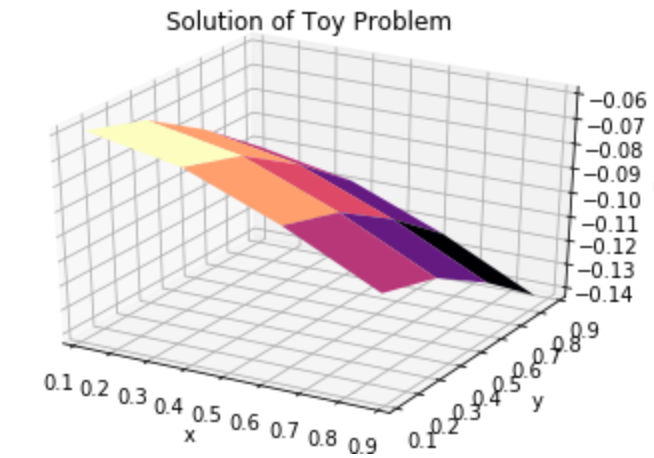
\includegraphics[width=\linewidth]{Materials/f4}
		\caption{Solution when the grid $f = X^4+Y^4$.}
		\label{e1}
	\end{subfigure}
	\hfill
	\begin{subfigure}[b]{0.45\linewidth}
		\centering
		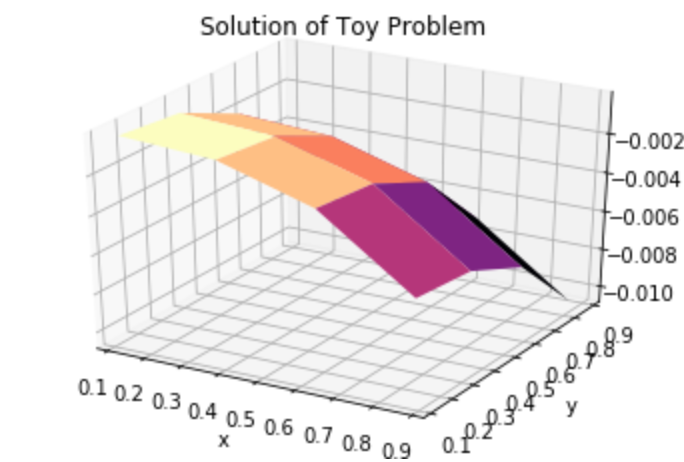
\includegraphics[width=\linewidth]{Materials/f4k10}
		\caption{Solution when the grid $f = X^4+Y^4$ and $\kappa = 10$.} 
		\label{e2}
	\end{subfigure}
	\begin{subfigure}[b]{0.45\linewidth}
		\centering
		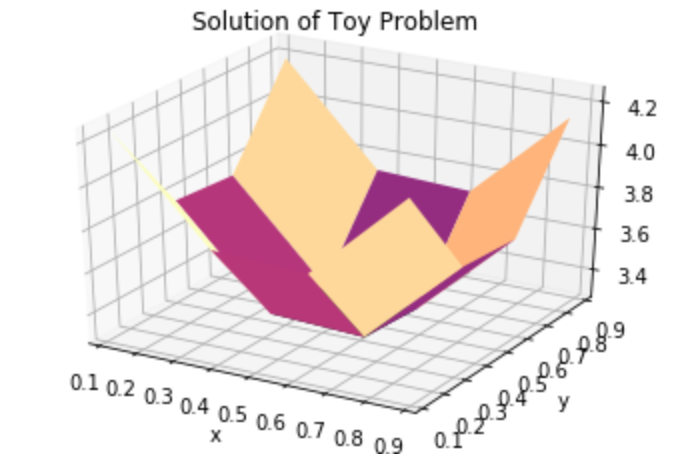
\includegraphics[width=\linewidth]{Materials/b=1}
		\caption{Solution when the grid $f = X+Y$, $\kappa = 2$ and von Neumann conditions equal 1.} 
		\label{e3}
	\end{subfigure}
	\hfill
	\begin{subfigure}[b]{0.45\linewidth}
		\centering
		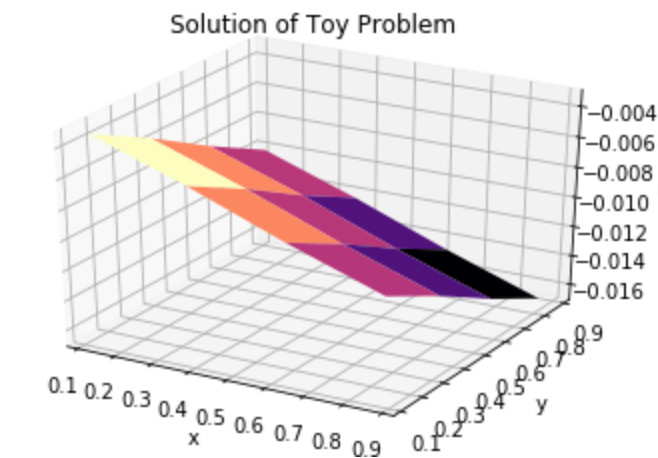
\includegraphics[width=\linewidth]{Materials/k10}
		\caption{Solution when the grid $f = X+Y$ and $\kappa = 10$.\\\hfill} 
		\label{e4}
	\end{subfigure}
\end{figure} 
As another experiment, we can look at the time it takes to solve $\mathbf{Au} = \mathbf{f}$ for bigger and bigger square grids. We can do this by doing the matrix assembly and then time how long it takes numpy to perform \textit{np.linalg.solve}. We do this over 10 iteration where we solve the same system and then take the average of the times to avoid some of the variance of how many resources the computer has available at the time of the computation. In \autoref{runtime} we see that the time to solve the linear system grows exponentially as we increase the grid size. This is not entirely surprising as the number of grid cells in a square grid also grows exponentially, and so as we increase the grid size the $\mathbf{Au}$ matrix grows exponentially in size.

\begin{figure}[H]
	\centering
	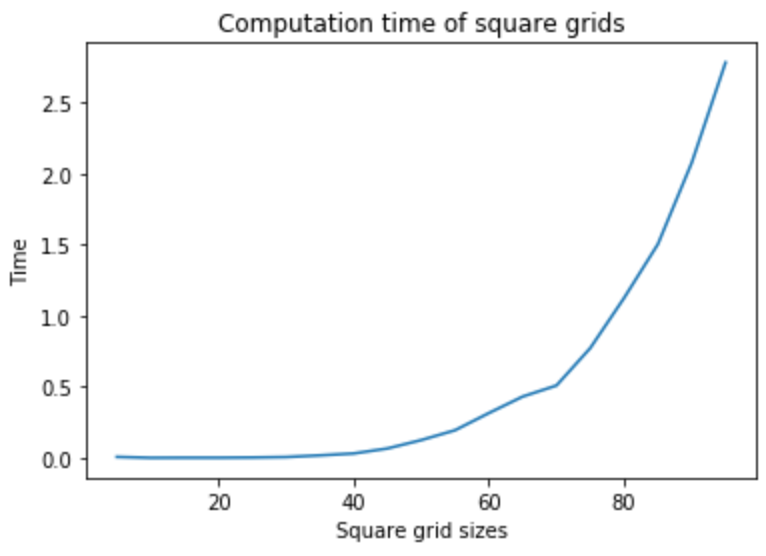
\includegraphics[width=0.6\linewidth]{Materials/runtime}
	\caption{Graph of how long it takes to solve the linear system vs. size of a square grid.}
	\label{runtime}
\end{figure}